\documentclass{article}
\usepackage{physics}
\usepackage{graphicx}
\usepackage{caption}
\usepackage{amsmath}
\usepackage{bm}
\usepackage{framed}
\usepackage{authblk}
\usepackage{empheq}
\usepackage{amsfonts}
\usepackage{esint}
\usepackage[makeroom]{cancel}
\usepackage{dsfont}
\usepackage{centernot}
\usepackage{mathtools}
\usepackage{subcaption}
\usepackage{bigints}
\usepackage{amsthm}
\theoremstyle{definition}
\newtheorem{lemma}{Lemma}
\newtheorem{defn}{Definition}[section]
\newtheorem{prop}{Proposition}[section]
\newtheorem{rmk}{Remark}[section]
\newtheorem{thm}{Theorem}[section]
\newtheorem{exmp}{Example}[section]
\newtheorem{prob}{Problem}[section]
\newtheorem{sln}{Solution}[section]
\newtheorem*{prob*}{Problem}
\newtheorem{exer}{Exercise}[section]
\newtheorem*{exer*}{Exercise}
\newtheorem*{sln*}{Solution}
\usepackage{empheq}
\usepackage{tensor}
\usepackage{xcolor}
%\definecolor{colby}{rgb}{0.0, 0.0, 0.5}
\definecolor{MIT}{RGB}{163, 31, 52}
\usepackage[pdftex]{hyperref}
%\hypersetup{colorlinks,urlcolor=colby}
\hypersetup{colorlinks,linkcolor={MIT},citecolor={MIT},urlcolor={MIT}}  
\usepackage[left=1in,right=1in,top=1in,bottom=1in]{geometry}
\setcounter{MaxMatrixCols}{20}
\usepackage{newpxtext,newpxmath}
\newcommand*\widefbox[1]{\fbox{\hspace{2em}#1\hspace{2em}}}

\newcommand{\p}{\partial}
\newcommand{\R}{\mathbb{R}}
\newcommand{\C}{\mathbb{C}}
\newcommand{\lag}{\mathcal{L}}
\newcommand{\nn}{\nonumber}
\newcommand{\ham}{\mathcal{H}}
\newcommand{\M}{\mathcal{M}}
\newcommand{\I}{\mathcal{I}}
\newcommand{\K}{\mathcal{K}}
\newcommand{\F}{\mathcal{F}}
\newcommand{\w}{\omega}
\newcommand{\lam}{\lambda}
\newcommand{\al}{\alpha}
\newcommand{\be}{\beta}
\newcommand{\x}{\xi}

\newcommand{\G}{\mathcal{G}}

\newcommand{\f}[2]{\frac{#1}{#2}}

\newcommand{\ift}{\infty}

\newcommand{\lp}{\left(}
\newcommand{\rp}{\right)}

\newcommand{\lb}{\left[}
\newcommand{\rb}{\right]}

\newcommand{\lc}{\left\{}
\newcommand{\rc}{\right\}}


\newcommand{\V}{\mathbf{V}}
\newcommand{\U}{\mathcal{U}}
\newcommand{\Id}{\mathcal{I}}
\newcommand{\D}{\mathcal{D}}
\newcommand{\Z}{\mathcal{Z}}

%\setcounter{chapter}{-1}


\usepackage{enumitem}



\usepackage{listings}
\captionsetup[lstlisting]{margin=0cm,format=hang,font=small,format=plain,labelfont={bf,up},textfont={it}}
\renewcommand*{\lstlistingname}{Code \textcolor{violet}{\textsl{Mathematica}}}
\definecolor{gris245}{RGB}{245,245,245}
\definecolor{olive}{RGB}{50,140,50}
\definecolor{brun}{RGB}{175,100,80}

%\hypersetup{colorlinks,urlcolor=colby}
\lstset{
	tabsize=4,
	frame=single,
	language=mathematica,
	basicstyle=\scriptsize\ttfamily,
	keywordstyle=\color{black},
	backgroundcolor=\color{gris245},
	commentstyle=\color{gray},
	showstringspaces=false,
	emph={
		r1,
		r2,
		epsilon,epsilon_,
		Newton,Newton_
	},emphstyle={\color{olive}},
	emph={[2]
		L,
		CouleurCourbe,
		PotentielEffectif,
		IdCourbe,
		Courbe
	},emphstyle={[2]\color{blue}},
	emph={[3]r,r_,n,n_},emphstyle={[3]\color{magenta}}
}

\newcommand{\diag}{\text{diag}}
\newcommand{\psirot}{\ket{\psi_\text{rot}(t)} }
\newcommand{\RWA}{\ham_\text{rot}^\text{RWA}}

% 3j symbol
\newcommand{\tj}[6]{ \begin{pmatrix}
		#1 & #2 & #3 \\
		#4 & #5 & #6 
\end{pmatrix}}


\begin{document}
\begin{framed}
\noindent Name: \textbf{Huan Q. Bui}\\
Course: \textbf{8.421 - AMO I}\\
Problem set: \textbf{\#11}\\
Due: Monday, May 2, 2022.
\end{framed}




\noindent \textbf{1. Scattering of light by a trapped atom.} Here we look at the matrix element involved in the scattering of light by a trapped atom. The light field propagates in the $x$ direction and has phase factor $e^{ikx}$. In quantum mechanics, this is a momentum displacement operator -- translating by $\hbar k$ in momentum space -- generating photon (or rather, \textit{atom}) recoil. Suppose that the wavefunctions for the initial and final motional state of the atom are $\psi_i(x)$ and $\psi_f(x)$. The matrix element is 
\begin{align*}
\bra{\psi_f(x)} e^{ikx} \ket{\psi_i(x)} = \int dx\,  \psi_f^*(x) e^{ikx} \psi_i(x) 
\end{align*} 

\begin{enumerate}[label = (\alph*)]
	\item Going to momentum space, we have 
	\begin{align*}
	\phi_{i,f}(p) =  \f{1}{\sqrt{2\pi }} \int dx\, e^{-ipx}\psi_{i,f}(x). 
	\end{align*}
	where we have used the \textit{symmetric} definition of the Fourier transform rather than the one given in the statement of the problem\footnote{Only because it is nicer and we don't have to worry about where the factor $(2\pi)^{\pm d/2}$ goes...}.  With this, we find 
	\begin{align*}
	\bra{\phi_f(p+k)} \ket{\phi_i(p)} 
	&=  \int dp\, \phi_f^*(p+k) \phi_i(p) \\
	&= \f{1}{2\pi}\int  dp\, \lp \int dx\, e^{+i(p+k)x}\psi_{f}^*(x)\rp \lp \int dx\, e^{-ipx'}\psi_{i}(x')\rp \\
	&= \f{1}{2\pi} \int dx \, \psi_f^*(x) e^{ikx} \int dx'\, \psi_i(x') \int dp\, e^{ip(x-x')} \\
	&=  \int dx \, \psi_f^*(x) e^{ikx} \int dx'\, \psi_i(x') \delta(x-x')\\
	&= \int dx\, \psi_f^*(x) e^{ikx}\psi_i(x)\\
	&= \bra{\psi_f(x)} e^{ikx} \ket{\psi_i(x)}
	\end{align*}
	as desired. 
	
	
	\item Consider a harmonically trapped atom of mass $M$ where the trapping frequency is $\omega$. Assume further that the ground and excited state experiences the same harmonic trap. We will evaluate the matrix element 
	\begin{align*}
	\bra{m} e^{ikx} \ket{n}
	\end{align*}
	where $m,n$ are the quantum numbers in the initial and final harmonic oscillator state of the scattering process. Here, 
	\begin{align*}
	\psi_n(x) = \bra{x}\ket{n} = \f{1}{\sqrt{2^n n! \sqrt{\pi}}} \exp\lp -\f{M\omega x^2}{2\hbar} \rp H_n\lp \sqrt{\f{M\omega}{\hbar}} x \rp
	\end{align*}
	and $\phi_n(p)$ has the exact same form but with $x\to p/M\omega$:
	\begin{align*}
	\phi_n(p) = \bra{p}\ket{n} = \f{1}{\sqrt{2^n n! \sqrt{\pi}}} 
	\exp\lp -\f{p^2}{2M\hbar\omega} \rp H_n\lp \sqrt{\f{1}{M \hbar \omega}} p \rp.
	\end{align*}
	However, it is easier to use ladder operators to obtain analytical results. Let us  write\footnote{There appears to be a typo in the definition of $p$ in terms of $a$ and $a^\dagger$ in the problem statement. I am using the correct definition here.} By writing 
	\begin{align*}
	x &= x_0 (a+ a^\dagger) \\
	p &= -ix_0 M\omega (a - a^\dagger) 
	\end{align*}
	where $x_0 = \sqrt{\hbar/2M\omega}$ is a measure of the harmonic oscillator ground state size, we can disentangle $e^{ikx}$ as follows:
	\begin{align*}
	{e^{ikx}} = e^{ikx_0(a+a^\dagger)} = e^{ikx_0 a} e^{ikx_0 a^\dagger} e^{-ikx_0[a,a^\dagger]/2}
	= {e^{(kx_0)^2/2} e^{ikx_0 a} e^{ikx_0 a^\dagger}}
	\end{align*}
	Here we have used the fact that $a,a^\dagger$ commute with $[a,a^\dagger] =  \mathbb{I}$ and the identity
	\begin{align*}
	e^{A+B} = e^{A} e^B e^{-[A,B]/2} 
	\end{align*}
	for operators $A,B$ which commute with $[A,B]$. 
	
	
	\item With
	\begin{align*}
	&a^1\ket{n} = \sqrt{n} \ket{n-1} \\
	&a^2\ket{n} = a\sqrt{n}\ket{n-1} = \sqrt{n(n-1)}\ket{n-2}\\
	&a^3\ket{n} = a^2\sqrt{n}\ket{n-1} = a\sqrt{n(n-1)}\ket{n-2} = \sqrt{n(n-1)(n-2)}\ket{n-3}\\
	&\vdots
	\end{align*}
	we have 
	\begin{align*}
	a^j\ket{n} = 
	\begin{cases}
	\sqrt{\f{n!}{(n-j)!}} \ket{n-j}, &\quad\quad j \leq n\\
	0, &\quad\quad \text{otherwise.}
	\end{cases}
	\end{align*}
	With this, we find
	\begin{align*}
	e^{ikx_0 a}\ket{n} 
	&= \sum_j \f{(ikx_0)^j a^j}{j!}\ket{n} \\
	&= \sum_j \f{(ikx_0)^j }{j!} \sqrt{\f{n!}{(n-j)!}} \ket{n-j}.
	\end{align*}
	
	
	\item Using the result we will calculate $\bra{m} e^{ikx} \ket{n}$. To do this, first assume that $m \leq n$. Define $\Delta n = n-m$.  Following a similar line of reasoning in (b)\footnote{by writing $x\sim a^\dagger + a$ instead of $a+a^\dagger$} we find that $
	e^{ikx} = e^{-(kx_0)^2/2} e^{ikx_0 a^\dagger} e^{ikx_0 a}$. From here, we plug the result from Part (c) and obtain 
	\begin{align*}
	\bra{m} e^{ikx} \ket{n} 
	&= e^{-(kx_0)^2/2} \bra{m} e^{ikx_0 a^\dagger } e^{ikx_0 a}  \ket{n} \\
	&= e^{-(kx_0)^2/2} \sum_{l=0}^m \f{(-ikx_0)^l}{l!} \sqrt{\f{m!}{(m-l)!}} \bra{m-l} \sum_{j=0}^n \f{(ikx_0)^j}{j!} \sqrt{\f{n!}{(n-j)!}} \ket{n-j}\\
	&= e^{-(kx_0)^2/2} \sum^m_{l=0}\sum^n_{j=0} \delta_{m-l, n-j} \f{(-1)^l (ik x_0)^{l+j}}{l!j!} \sqrt{\f{m!n!}{(m-l)!(n-j)!}}. 
	\end{align*}
	Notice that each summand is nonzero only when $m-l = n-j \iff j = \Delta n + l$. So, 
	\begin{align*}
	\bra{m} e^{ikx} \ket{n}  
	&= e^{-(kx_0)^2/2}\sum^m_{l=0}\f{(-1)^l (ik x_0)^{2l + \Delta n}}{l!(\Delta n + l)!} \sqrt{\f{m!n!}{(m-l)!(m-l )!}} \\
	&= e^{-(kx_0)^2/2} \sqrt{\f{m!}{n!}} (ikx_0)^{\Delta n} \sum^m_{l=0} (-1)^l \f{n!}{(m-l)!(n-m + l)!} \f{(kx_0)^{2l}}{l!}\\
	&= e^{-(kx_0)^2/2} \sqrt{\f{m!}{n!}}(ikx_0)^{\Delta n} L^{\Delta n}_{m} [(kx_0)^2]
	\end{align*}
	where 
	\begin{align*}
	L^{\al}_\be(X) = \sum^{\be}_{q=0} (-1)^q {{\be + \al}\choose{\be - q}}\f{X^q}{q!}.
	\end{align*}
	Similarly, if $n \leq m$, then we would proceed similarly, except that we would pick the summation index to be $j$ rather than $l$. In this case by defining $\Delta n = m-n$ we would get a similar result, but with $m\leftrightarrow n$. In any case, with $\Delta n = \abs{n-m}$, we have 
	\begin{align*}
	\bra{m} e^{ikx}\ket{n} = \exp\lp -\f{(kx_0)^2}{2} \rp  \sqrt{\f{n_<!}{n_>!}} (ikx_0)^{\Delta n} L_{n_<}^{\Delta n}[(kx_0)^2],
	\end{align*}
	as desired. 
	
	\item We are interested in the case where $m,n \gg 1$. From the asymptotic behavior of the generalized Laguerre polynomials, we have
	\begin{align*}
	L^{\Delta n}_{n_<}[(kx_0)^2] \to \lp \f{n_<}{(kx_0)^2} \rp^{\Delta n / 2} e^{(kx_0)^2/2} J_{\Delta n} \lp 2\sqrt{n_< (kx_0)^2}\rp 
	\end{align*}
	where $J_\al(x)$ is the Bessel function. So, for $m,n \gg 1$, the matrix element is 
	\begin{align*}
	\abs{\bra{m} e^{ikx} \ket{n}}^2 = (n_<)^{\Delta n} \f{n_<!}{n_>!} J^2_{\Delta n}\lp 2 \sqrt{n} kx_0 \rp \to J^2_{\Delta n} \lp 2\sqrt{n} kx_0 \rp.
	\end{align*}
	Now, since $n\hbar \omega\sim M\omega^2 x_{\text{cl}}^2/2$, the energy of a classical harmonic oscillator, we have
	\begin{align*}
	2\sqrt{n} k x_0 = 2k \sqrt{\f{n \hbar \omega}{2M\omega^2}} = kx_\text{cl} \equiv \be.
	\end{align*}
	So, 
	\begin{align*}
	\abs{\bra{m} e^{ikx} \ket{n}}^2  = J^2_{\Delta n}(\be),
	\end{align*}
	as desired. 
	
\end{enumerate}

\noindent \textbf{2. Saturation Spectroscopy.}

\begin{enumerate}[label = (\alph*)]
	\item \textbf{Homogeneous broadening.} Here we consider  a dilute gas of density $n$ composed of atoms with resonant frequency $\omega_0$ and linewidth $\Gamma$. The gas is exposed to monochromatic light $\omega_L = \omega_0 + \delta$ and intensity $I = sI_\text{SAT}$. Assuming zero temperature. From Problem Set \#10\footnote{where we looked for the steady-state solution to the optical Bloch equation with spontaneous emission}, we know that the density of atoms in the excited state is 
	\begin{align*}
	n_2 = \lp \f{s/2}{1 + 4\delta^2/\Gamma^2 + s} \rp n 
	\end{align*}
	and therefore the density of atoms in the ground state is 
	\begin{align*}
	n_1 = n - n_2 = \lp 1- \f{s/2}{1 + 4\delta^2/\Gamma^2 + s} \rp n
	\end{align*}
	The absorption cross-section can be obtained from conservation of energy. The net rate of energy absorption per unit volume is given by absorption due to atoms in the ground state minus stimulated emission due to atoms in the excited state. Since the system is in steady state, the net rate of energy absorbed must be equal to the net rate of energy scattering out of the beam due to spontaneous emission. With this information, we have the following equation:
	\begin{align*}
	(n_1 - n_2)\sigma(\omega_L) I(\omega_L) = n_2 \Gamma \hbar \omega_L \implies \sigma(\omega_L) &= \f{n_2 \hbar \omega_L}{(n_1  - n_2) I(\omega_L)} \\
	&= \f{\Gamma^2/4}{\delta^2 + \Gamma^2/4} \f{s}{2} \f{\hbar \omega_L}{I(\omega_L)} \\
	&= \f{\Gamma^2/4}{\delta^2 + \Gamma^2/4} \f{s}{2} \f{\hbar \omega_L}{sI_\text{SAT}(\omega_L)} \\
	&= \f{\Gamma^2/4}{\delta^2 + \Gamma^2/4}  \f{\hbar \omega_L}{2I_\text{SAT}} \\
	&= \sigma_0 \f{\Gamma^2/4}{\delta^2 + \Gamma^2/4},
	\end{align*}
	where $\sigma_0 = $ is the resonant absorption cross section, $\sigma_0 = \lambda_0^2/2\pi$.\\
	
	
	
	The gas is in a box of length $L$ in the direction of the incoming light. The fraction of the light absorbed is given by 
	\begin{align*}
	\f{I(\omega_L, L)}{I(\omega_L,0)} = e^{-(n_1 - n_2)\sigma(\omega_L)L} = \exp\lb -\f{\Gamma^2/4}{\delta^2+(1+s)\Gamma^2/4} L n \sigma_0 \rb. 
	\end{align*}
	
	\item \textbf{The Bennet hole.} Suppose the atoms have mass $m$ and are at temperature $T$. Let the incoming light have a wavevector $\bm{k_L}$ along the $z$-axis. The population density distribution in the ground state $n_1(v_z)$ as a function of $v_z$ is given by the Maxwell-Gaussian velocity distribution minus some population due to excitation into the excited state. Without the incoming light, we have
	\begin{align*}
	n_1(v_z) = n_1\sqrt{\f{m}{2\pi k_BT}} \exp\lp -\f{m v_z^2}{2k_BT} \rp = \f{n_1}{\al\sqrt{\pi}} \exp\lp -\f{v_z^2}{\al^2} \rp, \quad\quad \al = \sqrt{\f{2k_BT}{m}}.
	\end{align*}
	The light interacts with atoms with velocity
	\begin{align*}
	v_z = \f{\omega_L - \omega_0}{k_L},
	\end{align*}
	removing atoms from the ground state and put them in the excited state, \textit{burning a hole} in $n_1(v_z)$. The width and depth of this hole can be obtained from looking the population difference. This can be found just as before, except that the detuning is modified by the Doppler shift:
	\begin{align*}
	n_1(v_z) - n_2(v_z) = n(v_z)\lb 1 - \f{s\Gamma^2/4}{(\omega_L - \omega_0 - v_z k_L)^2 + \Gamma^2(1+s)/4} \rb,
	\end{align*}
	where $n(v_z)$ follows the Gaussian distribution: $n(v_z) = n/(\al\sqrt{\pi}) \exp\lp -v_z^2/\al^2 \rp$. From this we find that the width of the hole is:
	\begin{align*}
	\Delta \omega_\text{hole} = \Gamma\lp 1 + s \rp^{1/2} \implies \Delta v_z = \f{\Gamma\lp 1 + s \rp^{1/2} }{k_L}.
	\end{align*}
	And the depth is obtained by setting the detuning term to zero:
	\begin{align*}
	d_\text{hole} = \f{s}{1+s} n(v_z) \bigg\vert_{v_z = (\omega_L - \omega)/k_L}
	\end{align*}
	
	
	
	\item \textbf{Inhomogeneous broadening.} Now suppose  that we sweep $\omega_L$ and measure the (small)  absorption of the beam. The fraction of the light absorbed as a function of $s$ and $\delta$ and compare with its value at $s = 0$ is given by $e^{-f(s,\delta)}$ where
	\begin{align*}
	f(s,\delta) = L\int_{-\infty}^\infty dv_z\, \lb n_1(v_z) - n_2(v_z) \rb \sigma(\omega_L-v_z k_L) 
	\end{align*}
	where $L$ is the length of the box. This expression comes from the differential equation:
	\begin{align*}
	\f{dI}{dz} = -(n_1 - n_2)\sigma(\omega) I(\omega)
	\end{align*}
	but generalized to account for the distribution in $v$. Substituting results from the previous parts of this problem, we can write $f$ in terms of $s$ and $\delta = \omega_L - \omega_0$:
	\begin{align*}
	f(s,\delta)
	&= \sigma_0 L \int_{-\infty}^\infty dv_z\, n(v_z) \lb 1 - \f{s\Gamma^2/4}{(\delta - v_z k_L)^2 + \Gamma^2(1+s)/4} \rb \f{\Gamma^2/4}{(\delta - v_zk_L)^2 + \Gamma^2(1+s)/4} \\
	&= \sigma_0 L  \int_{-\infty}^\infty dv_z\,  n(v_z) \f{\Gamma^2/4}{(\delta - v_z k_L)^2 + \Gamma^2(1+s)/4}\\
	&= \sigma_0 L \int_{-\infty}^\infty dv_z\, \f{n}{\al\sqrt{\pi}} \exp\lp -\f{v_z^2}{\al^2} \rp \f{\Gamma^2/4}{(\delta - v_z k_L)^2 + \Gamma^2(1+s)/4}\\
	&=  \f{\sigma_0 L}{1+s} \int_{-\infty}^\infty dv_z\, \f{n}{\al\sqrt{\pi}} \exp\lp -\f{v_z^2}{\al^2} \rp \f{\Gamma'^2/4}{(\delta - v_z k_L)^2 + \Gamma'^2/4}\\
	\end{align*}
	where $\Gamma' = \Gamma\sqrt{1+s}$. Here, $f(s,\delta)$ may be written in terms of the Voigt profile:
	\begin{align*}
	f(s,\delta) = \f{1}{1+s}V(\delta, \al, \Gamma').
	\end{align*}
	When $s=0$, this has value:
	\begin{align*}
	f(0,\delta) =  \sigma_0 L \int_{-\infty}^\infty dv_z\, \f{n}{\al\sqrt{\pi}} \exp\lp -\f{v_z^2}{\al^2} \rp \f{\Gamma^2/4}{(\delta - v_z k_L)^2 + \Gamma^2/4} = V(\delta,\al,\Gamma).
 	\end{align*}
	For high temperatures $(k_L \bar{v}_z) \gg \Gamma$, the Gaussian distribution is much wider compared to the Lorentzian profile. As a result, the Lorentzian acts as a delta-function which picks out atoms moving with velocity
	\begin{align*}
	v_z = \f{\omega_L - \omega_0}{k_L} = \f{\delta}{k_L}.
	\end{align*}
	By inspection, the absorption line is a Gaussian and has the form\footnote{Here I have admitted cheated a little by taking $k_L \approx k_0 = \omega_0/c$. This is okay in practice since $|\omega_L-\omega_0|$ is typically very small compared to $\omega_L$ and $\omega_0$. }
	\begin{align*}
	g_D(\omega_L) = \f{c}{\al \omega_0 \sqrt{\pi}} \exp\lb -\f{c^2}{\al^2}\lp \f{\omega - \omega_0}{\omega_0} \rp^2 \rb.
	\end{align*}
	From here we see that the width of the absorption line is the FWHM of this distribution:
	\begin{align*}
	\Delta \omega_D  = 2\sqrt{\ln 2} \f{\omega_0 \al}{c} \approx 1.7 \f{\omega_0 \al}{c},
	\end{align*}
	which does not depend on the saturation parameter. 
	
	
	\item \textbf{Saturation spectroscopy.} To actually get some benefit from saturating the gas, we introduce a second laser beam.
	\begin{enumerate}[label=(\roman*)]
		\item Now we add a weak counter-propagating probe beam at frequency $\omega_p$ with wavevector $k_p$. The absorption of this beam, including the effects of saturating due to $(\omega_L, k_L)$ is given by 
		\begin{align*}
		f(s,\omega_L, \omega_p) 
		&= \sigma_0 L \int dv_z\, \underbrace{[n_1(v_z) - n_2(v_z)]}_{\text{due to saturating $(\omega_L,k_L)$}} \times  \underbrace{\sigma(\omega_p + v_z k_p)}_{\text{abs. cx-section for $(\omega_p, k_p)$}}\\
		&= \sigma_0 L \int dv_z  \lb 1 - \f{s\Gamma^2/4}{(\omega_L - \omega_0 - v_z k_L)^2 + \Gamma^2(1+s)/4} \rb \f{n(v_z) \Gamma^2/4}{(\omega_p - \omega_0 + v_zk_p)^2 + \Gamma^2/4},
		\end{align*}
		where we have used the fact that the probe beam is weak, and therefore does not modify the population difference created by the pump beam.\\
		
		
		How to obtain absorption line shape and dip location? It is not easy to evaluate this integral. However, based on the form of the integrand (and also the physical setting) we expect that there is a dip in the absorption of the probe light when its frequency is 
		\begin{align*}
		\omega_{p,\text{dip}} = \omega_0 - (\omega_L - \omega_0) k_p/k_L.
		\end{align*}
		The width of the dip at $\omega_p = \omega_{p, \text{dip}}$ has equal contributions coming from the width of the Bennet hole and the natural linewidth of the atom. Therefore, 
		\begin{align*}
		\Gamma_p = \Gamma + \sqrt{1+s} \Gamma = \Gamma\lp 1+ \sqrt{1+s}\rp.
		\end{align*}
		
		
		\begin{figure}[!htb]
			\centering
			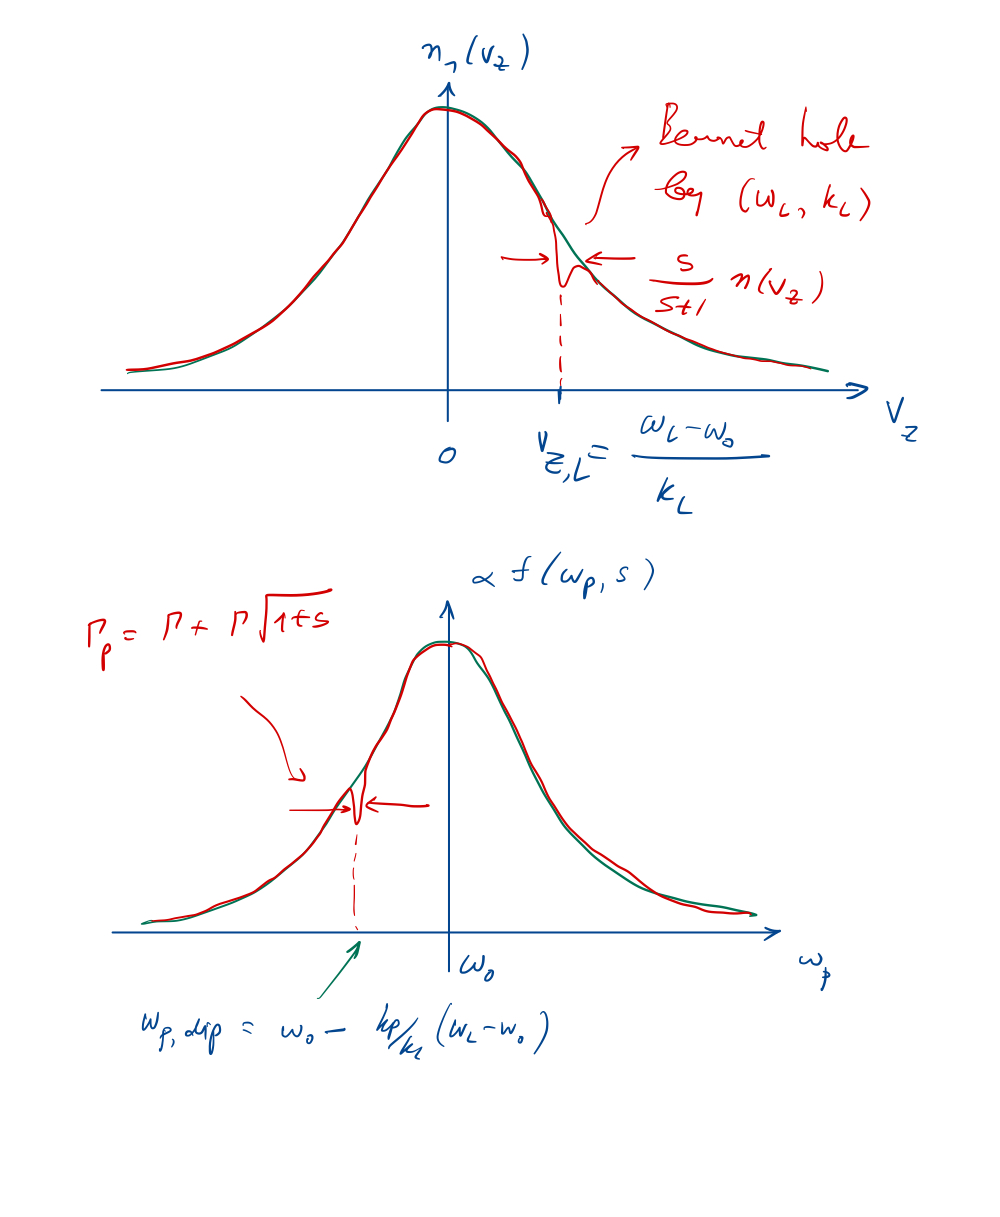
\includegraphics[width=0.52\textwidth]{2di}
			\caption{Absorption line shapes for various $\omega_p$'s.}
		\end{figure}
		
		
		
		 \newpage
		
		\item We can also just retroreflect the original beam. In this case, we have $\omega_L = \omega_p = \omega$ and $k_L = -k_p = k$. Assume that both beams have the same intensity $I$. Following what we did in Problem Set \#10 and the previous parts of the problem, we simply add another contribution to the population difference due to the (strong) probe beam:
		\begin{align*}
		n_1(v_z) - n_2(v_z) = n(v_z)\lb 1 - \f{s\Gamma^2/4}{(\omega - \omega_0 - v_z k)^2 + \Gamma^2(1+s)/4} - \f{s\Gamma^2/4}{(\omega-\omega_0 + v_z k)^2 + \Gamma^2(1+s)/4} \rb,
		\end{align*}
		We see that two Bennet holes are burned into $n_1(v_1)$ at $v_z = \pm |\omega - \omega_0|/k$. In the case that $\omega = \omega_0$, there is only one Bennet hole burned, which is located at the center of the distribution $v_z =0 $. For $\omega\neq\omega_0$, the depth of each Bennet hole is just as before:
		\begin{align*}
		d_{\text{hole}, \omega \neq \omega_0} = \f{s}{s+1}n(v_z)\bigg\vert_{v_z = \pm |\omega - \omega_0|/k}.
		\end{align*}
		When $\omega = \omega_0$, however, the two Bennet holes combine at $v_z = 0$ and give
		\begin{align*}
		d_{\text{hole}, \omega = \omega_0} = \f{2s}{s+1}n(0).
		\end{align*}
		
		
		\begin{figure}[!htb]
			\centering
			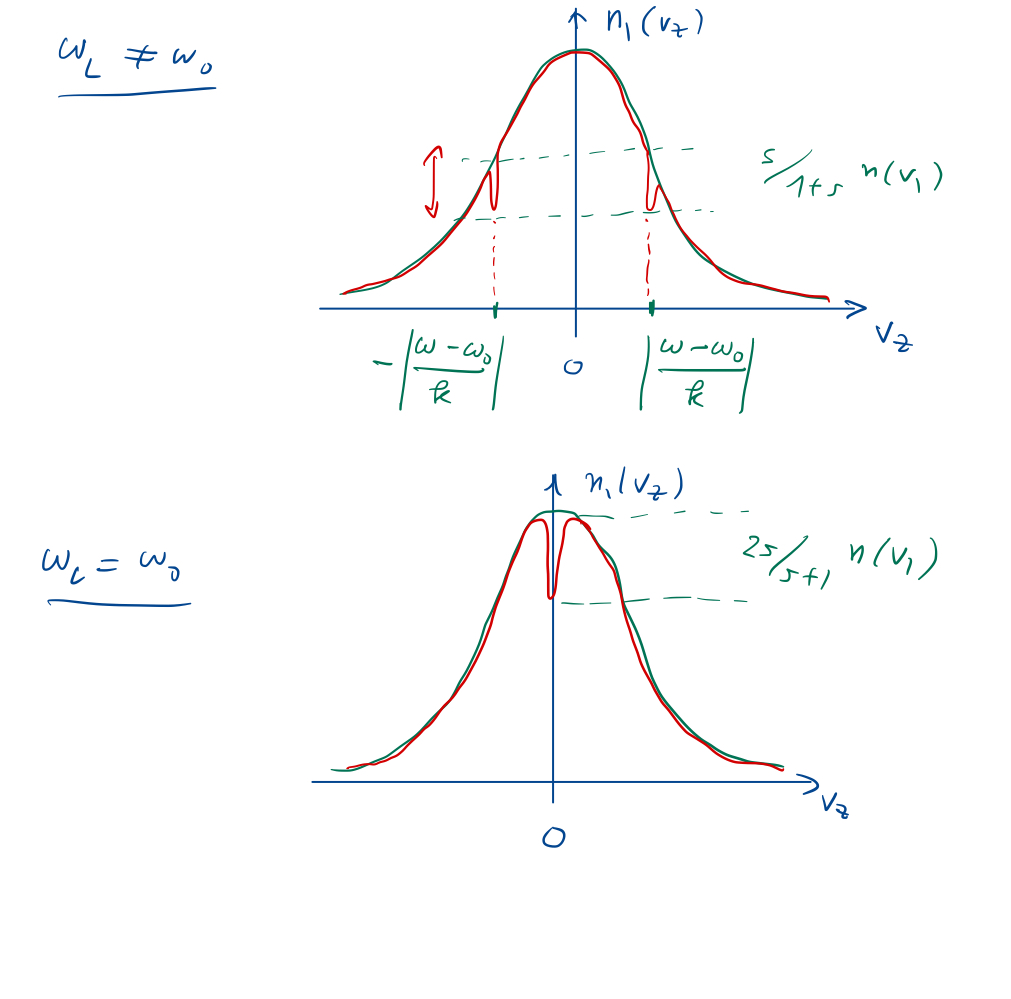
\includegraphics[width=0.75\textwidth]{2dii_1}
			\caption{$n_1(v_z)$ for $\omega \neq \omega_0$ and $\omega = \omega_0$}
		\end{figure}
		
		
		Now we want to look at the absorption profile for the retroreflected beam. The integrals involved here seem too complicated, so I don't think I can get into any of the math here. In any case, I suspect that the width of the central feature is dictated only by the natural linewidth and the saturation parameter. So the only reasonable guess is 
		\begin{align*}
		\Delta \omega_{\text{dip, retro}} = \Gamma\sqrt{1+s}.
		\end{align*}
		
		
		\begin{figure}[!htb]
			\centering
			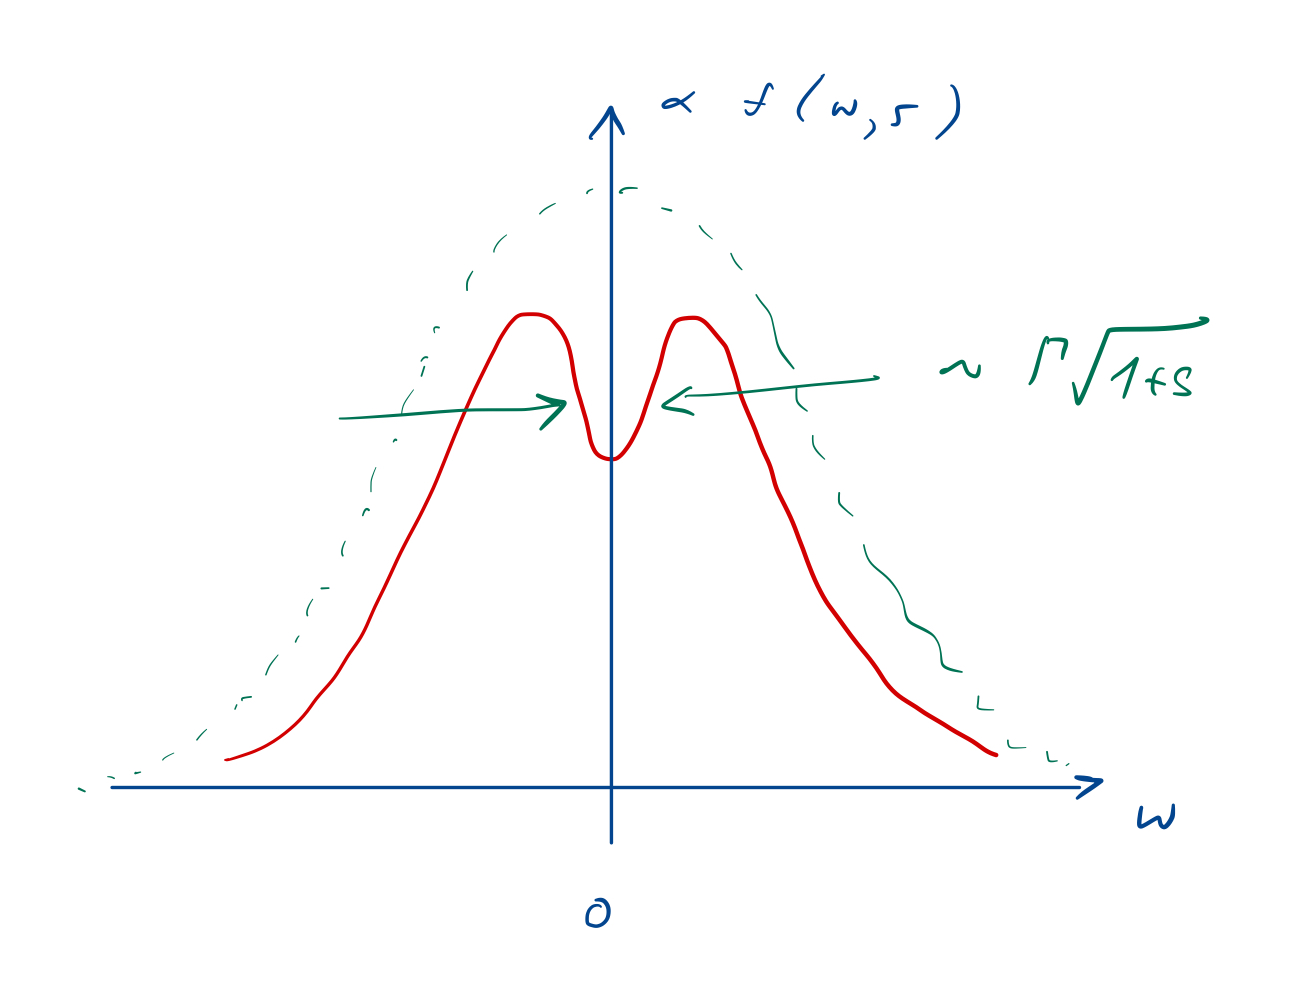
\includegraphics[width=0.7\textwidth]{2dii_2}
			\caption{Absorption of the retroreflected beam with central feature $\delta = 0$. }
		\end{figure}
		
		
	\end{enumerate}
\end{enumerate}
	
	
\end{document}








